\documentclass[x11names]{article}
\usepackage{tikz}
\usepackage{pgfplots}
\usepackage{xcolor}
\usepackage{svg}
\usepackage{amsmath}
\usepackage{array}
\usepackage[skins]{tcolorbox}
\usepackage[version=4]{mhchem}
\usepackage[a4paper, total={6in, 10in}]{geometry}
\usepackage{fouriernc}
\usepackage{xymtex}
\usepackage{textcomp}
\usepackage{eurosym}
\usepackage{mathrsfs}
\usepackage{float}
\usepackage{pst-all}
\usepackage{pst-3dplot}
\usepackage{leftindex}
\usepackage{verbatim}
\usepackage{import}
\usepackage{xifthen}
\usepackage{pdfpages}
\usepackage{transparent}
\usepackage{import}
\usepackage{pdfpages}
\usepackage{transparent}


\pdfsuppresswarningpagegroup=1
\newcommand{\incfig}[1]{%
    \def\svgwidth{\columnwidth}
    \import{./figures/}{#1.pdf_tex}
}



% myframe
\newtcolorbox{es}[2][]{%
  enhanced,colback=white,colframe=black,coltitle=black,
  sharp corners,boxrule=0.4pt,
  fonttitle=\itshape,
  attach boxed title to top left={yshift=-0.5\baselineskip-0.4pt,xshift=2mm},
  boxed title style={tile,size=minimal,left=0.5mm,right=0.5mm,
    colback=white,before upper=\strut},
  title=#2,#1
}

\newtcolorbox{blues}[2][]{%
  enhanced,colback=Azure2,colframe=black,coltitle=black,
  sharp corners,boxrule=0.4pt,
  fonttitle=\itshape,
  attach boxed title to top left={yshift=-0.5\baselineskip-0.4pt,xshift=2mm},
  boxed title style={tile,size=minimal,left=0.5mm,right=0.5mm,
    colback=Azure2,before upper=\strut},
  title=#2,#1
}

\newtcolorbox{defin}[2][]{%
  enhanced,colback=white,colframe=LightSkyBlue1,coltitle=black,
  sharp corners,boxrule=1.5pt,
  fonttitle=\itshape,
  attach boxed title to top left={yshift=-0.5\baselineskip-0.4pt,xshift=2mm},
  boxed title style={tile,size=minimal,left=0.5mm,right=0.5mm,
    colback=white,before upper=\strut},
  title=#2,#1
}


%% regole
\renewcommand*\contentsname{Indice}
\setcounter{tocdepth}{4}
\setcounter{secnumdepth}{2}
\pgfplotsset{compat=1.15}

\usetikzlibrary{arrows}


\title{Letteratura italiana}
\author{Federico Cesari}
\date{}



%% DOCUMENTO


\begin{document}

\begin{titlepage}
	\begin{center}
		\vspace*{1cm}
		
		\textbf{\LARGE Relazione di laboratorio - Pendolo semplice}
		
		\vspace{0.3cm}
		\large \textit{Misura del periodo di un pendolo semplice} \\
		
		\vspace{0.5cm}
		\Large Federico Cesari \\
		
		\small 1096759 
		\vspace{0.2cm}
		
		\small Gruppo 5
		
		
		\vspace{3cm}
		\begin{center}
			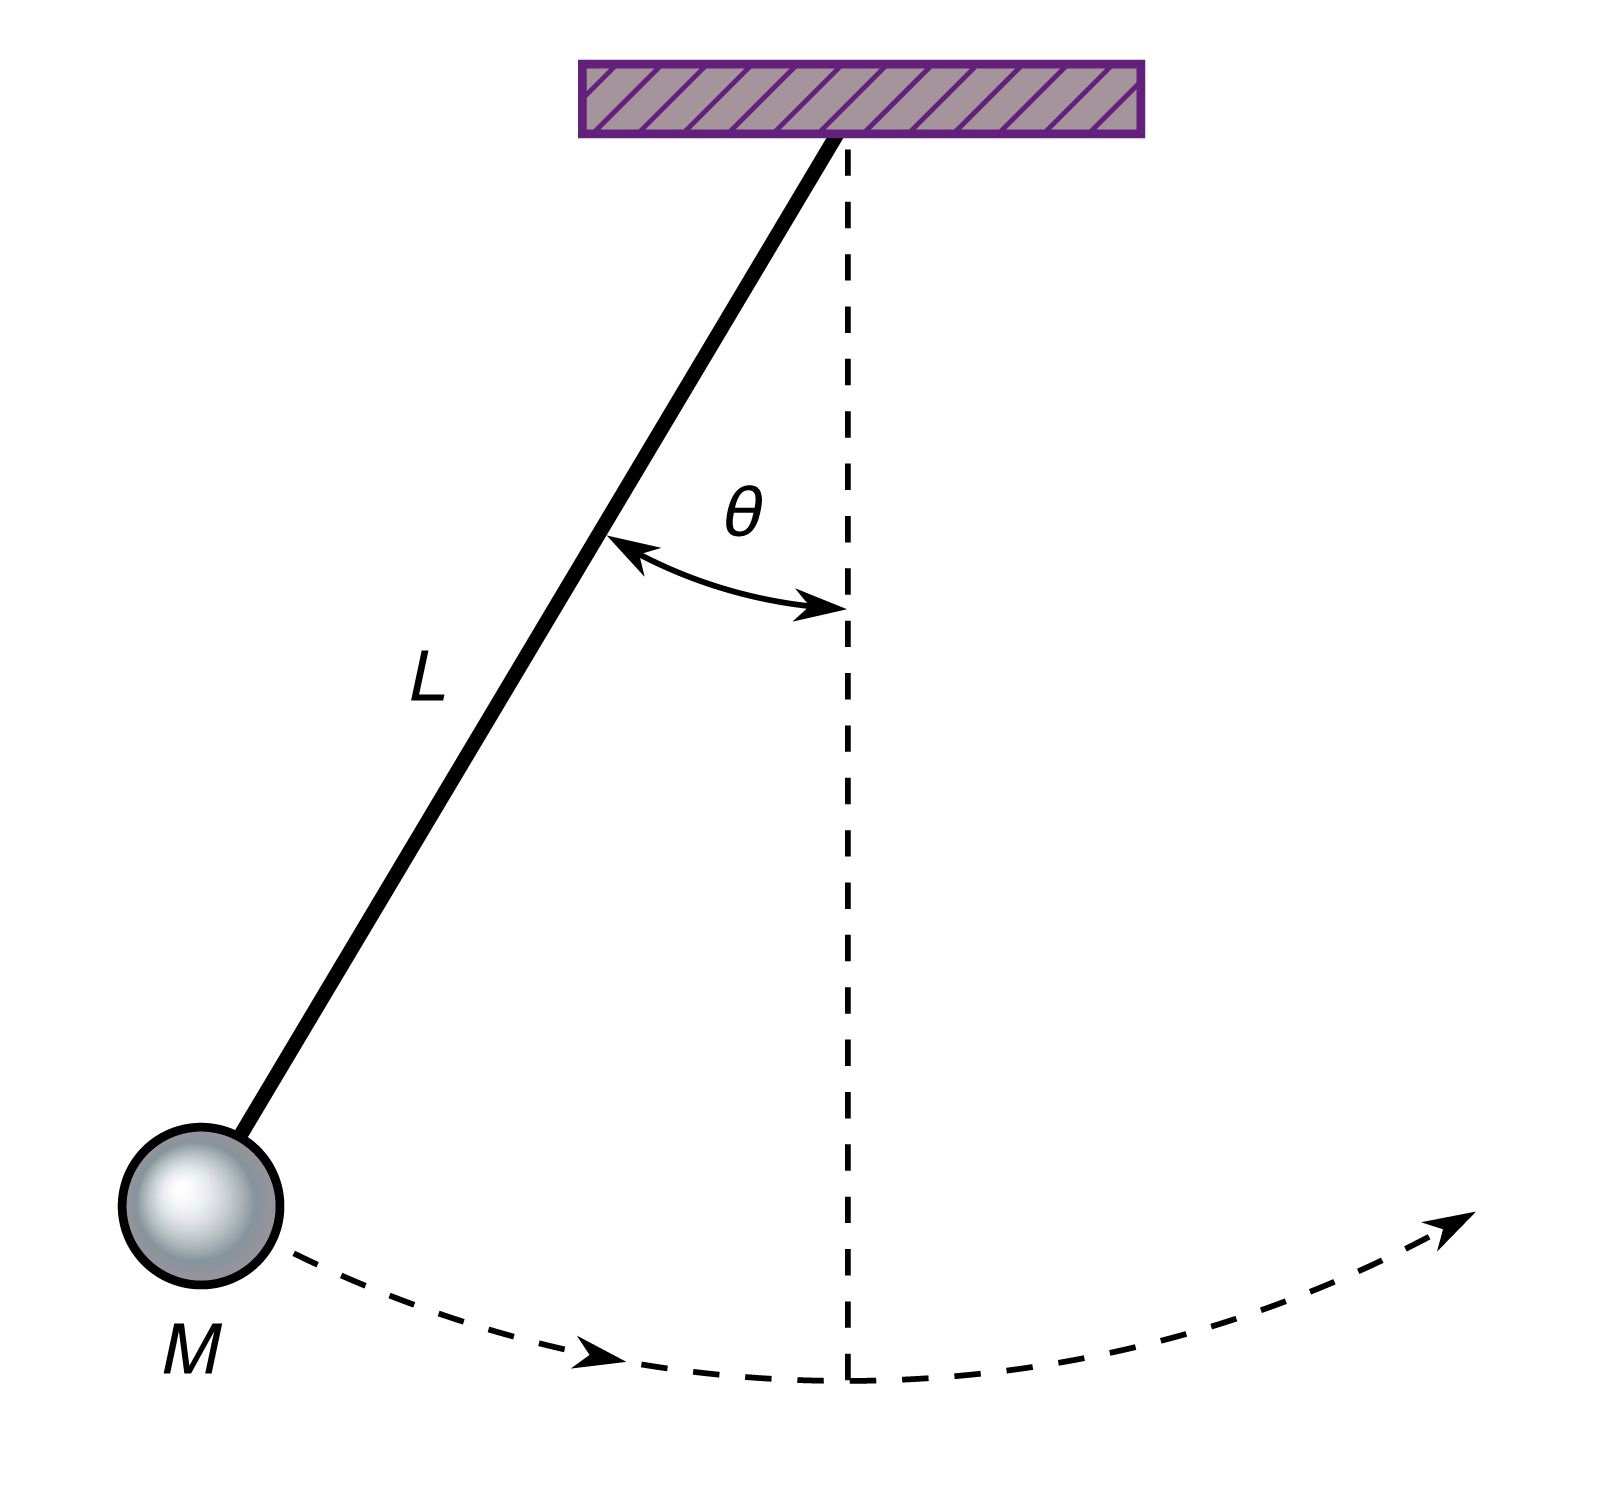
\includegraphics[scale=0.1]{IMG_0200.jpeg}	
		\end{center}
		
		
		
		\vfill
		
		
		
		corso A\\
		Università degli studi di Torino, Torino\\
		4 aprile 2024\\
		
		
	\end{center}
\end{titlepage}
\tableofcontents
\newpage

%%%%           %%%%
%     VETTORI     %
%%%%%          %%%%%%%%%%%%%%%%%%%%%%%%%%%%%%%%%%%%%%%%%%%%%%%%%%%%%%%%%%%%%%%%%%%
%%%%%%%%%%%%%%%%%%%%%%%%%%%%%%%%%%%%%%%%%%%%%%%%%%%%%%%%%%%%%%%%%%%%%%%%%%%%%%%%%%




















\newpage
\section{Spazi Vettoriali}
Possiamo vedere i vettori da diversi punti di vista, tutti validi, ma con intenti applicativi differenti. Possiamo definire vettori una freccia nello spazio caratterizzata da un modulo, una direzione e da un verso; oppure possiamo intendere un vettore una lista ordinata di numeri.

Se in fisica non importa la posizione nello spazio di un vettore, in algebra lineare questo sarà quasi sempre attaccato all'origine del nostro sistema di riferimento.

\begin{center}
\fboxsep11pt
\colorbox{Azure2}{\begin{minipage}{5.75in}
\begin{blues}{Definizione: Spazio Vettoriale}
    Si definisce \textbf{spazio vettoriale} sul campo dei numeri reali $\mathbb{R}$ un certo insieme $V$ nel quale sono definite le seguenti operazioni:
    \begin{enumerate}
        \item somma $+$: $V \times V \longrightarrow V$.
        \item prodotto $\cdot$: $\mathbb{R} \times V \longrightarrow V$.
        \end{enumerate}
	Un gruppo $\left(V,\times \right)$ si dice \textit{commutativo} (o Abeliano) se $v \times y = y \times x \quad \forall x,y \in V$
\end{blues}
\end{minipage}}        
\end{center}


\subsubsection{Proprietà della somma}
\begin{enumerate}
    \item commutativa: $x + y = y + x, \quad \forall x,y \in V$
    \item associativa: $(x+y)+z = x + (y+z),\quad \forall x,y \in V$
    \item esistenza dell'elemento neutro: $\exists 0 \in V : 0 + x = x +0, \quad \forall x,y \in V$
    \item esistenza dell'opposto: $\forall x \in V \exists -x \in V : x + (-x) = (-x) +x = 0$
\end{enumerate}
\subsubsection{Proprietà del prodotto}
\begin{enumerate}
    \item (diciamo) distributiva: $\lambda(x+y) = \lambda x + \lambda y,\quad \forall x,y \in V, \forall \lambda \in \mathbb{R}$
    \item $(\lambda + \mu)\cdot \overline{x} = \lambda \overline{x} + \mu \overline{x}, \quad \forall x,y \in V, \forall \lambda \in \mathbb{R}$
    \item $(\lambda \cdot \mu)\overline{x} = \lambda(\mu \cdot \overline{x}),\quad \forall x,y \in V$
    \item $1 \cdot \overline{x} = \overline{x}, \quad \forall x,y \in V$
\end{enumerate}



\subsection{Sottospazi vettoriali}
\begin{center}
\fboxsep11pt
\colorbox{Azure2}{\begin{minipage}{5.75in}
\begin{blues}{Definizione: sottospazio vettoriale}
Sia $V$ uno spazio vettoriale reale, $W \subseteq V $ è un sottospazio vettoriale di $V$ se $W$ è uno spazio vettoriale rispetto alle stesse operazioni di $V$, quindi rispetto alle operazioni di \textit{somma} e \textit{prodotto}.

\begin{itemize}
	\item Se ho 2 elementi $\overline{x},\overline{y}\in W \quad \Rightarrow \quad \overline{x} + \overline{y} \in W$;
	\item Se ho 2 elementi $\overline{x} \in W, \lambda \in \mathbb{R} \quad \Rightarrow \quad \lambda\overline{x} \in W$.
\end{itemize}

\end{blues}
\end{minipage}}        
\end{center}
\subsubsection{Esempi di sottospazi vettoriali}



Il piano $xy$ in questo caso si può dire essere un sottospazio vettoriale. Lo chiamiamo  $W$ e possiamo scrivere:


%%%%           %%%%
%     MATRICI     %
%%%%%          %%%%
\newpage
\section{Matrici}
\subsection*{Interpretazione geometrica delle matrici}
Dopo aver parlato di vettori, approfondiamo il concetto di \textit{matrice} e il suo comportamento come \textit{spazio vettoriale}. Più in particolare vedremo il prodotto tra matrici come trasformazioni lineari dello spazio vettoriale (linearmente perché nessuna linea viene curvata e l'origine rimane fissata). Questa interpretazione di una matrice rende i conti più facili ed intuitivi. 

\noindent
Diciamo di avere due vettori giacenti sui due assi:

\begin{center}
\begin{tikzpicture}[line cap=round,line join=round,>=triangle 45,x=1cm,y=1cm]
\begin{axis}[
x=1cm,y=1cm,
axis lines=middle,
ymajorgrids=true,
xmajorgrids=true,
xmin=-2,
xmax=2,
ymin=-2,
ymax=2,
ylabel={}, 
x tick label style={opacity=0},
y tick label style={opacity=0}]
\draw [->,line width=1pt,color=SteelBlue3] (0,0) -- (0,1);
\draw [->,line width=1pt,color=SlateBlue3] (0,0) -- (1,0);
\begin{scriptsize}
\draw[color=SteelBlue3] (-1,1) node {$\hat{y}=\begin{bmatrix}0\\1\end{bmatrix}$};
\draw[color=SlateBlue3] (1,0.5) node {$\hat{x}=\begin{bmatrix}1\\0\end{bmatrix}$};
\end{scriptsize}
\end{axis}
\end{tikzpicture}    
\end{center}

\noindent
Diciamo ora di avere una matrice $A$ che descrive dove questi due vettori cadono a seguito della trasformazione da essa descritta; la matrice $A$ basta per descrivere dove cadrà ogni vettore (x,y). 
$$
x=\begin{bmatrix}
    \textcolor{SlateBlue3}{1} & \textcolor{SteelBlue3}{3} \\
    \textcolor{SlateBlue3}{-2} & \textcolor{SteelBlue3}{0}
\end{bmatrix}
$$
$$
\begin{bmatrix}
   \textcolor{SlateBlue3}{1} & \textcolor{SteelBlue3}{3} \\
   \textcolor{SlateBlue3}{-2} & \textcolor{SteelBlue3}{0} 
\end{bmatrix}
\begin{bmatrix}
    x \\
    y
\end{bmatrix}
= x
\begin{bmatrix}
    \textcolor{SlateBlue3}{1} \\ \textcolor{SlateBlue3}{-2}
\end{bmatrix}
+ y
\begin{bmatrix}
    \textcolor{SteelBlue3}{3} \\ \textcolor{SteelBlue3}{0}
\end{bmatrix}
$$
\textit{Se, come abbiamo detto prima, le linee non vengono deformate, il vettore che nel primo grafico sarebbe stato (1,1), nel secondo è intuitivo pensare che ora sia (4,-2); Il prodotto tra le matrici lo conferma}.

\begin{center}
\begin{tikzpicture}[line cap=round,line join=round,>=triangle 45,x=1cm,y=1cm]
\begin{axis}[
x=1cm,y=1cm,
axis lines=middle,
ymajorgrids=true,
xmajorgrids=true,
xmin=-4,
xmax=4,
ymin=-4,
ymax=4,
ylabel={}]
\clip(-7.079913199747649,-3.637084505116807) rectangle (8.353685115497054,5.590837202953786);
\draw [->,line width=1pt,color=SteelBlue3] (0,0) -- (3,0);
\draw [->,line width=0.5pt,color=SkyBlue4] (0,0) -- (4,-2);
\draw [->,line width=1pt,color=SlateBlue3] (0,0) -- (1,-2);
\begin{scriptsize}
\draw[color=SteelBlue3] (2,0.6) node {$\hat{y}=\begin{bmatrix}3\\0\end{bmatrix}$};
\draw[color=SlateBlue3] (1.7,-1.5) node {$\hat{x}=\begin{bmatrix}1\\-2\end{bmatrix}$};
\end{scriptsize}
\end{axis}
\end{tikzpicture}    
\end{center}

\noindent
Possiamo arrivare alla conclusione che ogni matrice può essere interpretata come una trasformazione dello spazio, a prescindere dall'ordine della matrice.
\paragraph*{Prodotto come composizione di trasformazioni}
Se applichiamo più trasformazioni consecutive, quindi tramite più matrici, interpretiamo la composizione di queste trasformazioni come il prodotto tra le matrici.
$$
\begin{bmatrix}
    \textcolor{Brown2}{1} & \textcolor{Brown2}{1} \\
    \textcolor{Brown2}{0} & \textcolor{Brown2}{1} \\
\end{bmatrix}
\begin{bmatrix}
    \textcolor{SteelBlue3}{0} & \textcolor{SteelBlue3}{-1} \\
    \textcolor{SteelBlue3}{1} & \textcolor{SteelBlue3}{0} \\
\end{bmatrix}
=
\begin{bmatrix}
    1 & -1 \\
    1 & 0
\end{bmatrix}
$$

\noindent
L'ordine di composizione va letto da destra verso sinistra: viene eseguita prima la \textcolor{SteelBlue3}{blu}, poi la \textcolor{Brown2}{rossa} (cosa tipica delle notazione delle funzioni: $f(g(x))$).

\noindent
Pensando in questi termini, prodotto come composizione di trasformazioni, comprendiamo perché $AB \neq BA$; e la proprietà associativa diventa chiara e logica: $A(BC) = (AB)C$ in quanto l'ordine delle trasformazioni rimane invariato.


\subsection{Spazio vettoriale delle matrici}
Definiamo una matrice di $r$ righe e $n$ colonne con $a_{ij} \in \mathbb{R}; i = 1,\dots,r; j = 1,\dots,n$ definita nello spazio $\mathbb{R}^{rn}$ in questo modo:
$$
A=
\begin{bmatrix}\;a_{1,1}&a_{1,2}&\cdots &a_{1,n}\\\;a_{2,1}&a_{2,2}&\cdots &a_{2,n}\\\vdots &\vdots &\ddots &\vdots \\\;a_{r,1}&a_{r,2}&\cdots &a_{r,n}\end{bmatrix}
$$
Esistono matrici \textbf{quadrate} se hanno stesso numero di righe e di colonne ($\mathbb{R}^{nn}$), \textbf{diagonali} se tutti gli elementi sono zeri tranne quelli sulla diagonale maggiore (matrice \textit{unità} se la diagonale contiene solo $1$), \textbf{nulle} se tutti gli elementi sono zeri, \textbf{riga} se hanno una riga sola, \textbf{colonna} se hanno una colonna sola.

$$
\begin{bmatrix}1 & 1 & 0 \\ 0 & 1 & 2\\ 0 & 3 & 1\end{bmatrix}
\hspace{1cm}
\begin{bmatrix}1 & 0 & 0\\0 & 1 & 0\\ 0 & 0 & 1\end{bmatrix}
\hspace{1cm}
\begin{bmatrix}0 & 0 & 0\\0 & 0 & 0\\ 0 & 0 & 0\end{bmatrix}
\hspace{1cm}
\begin{bmatrix}1 & 2 & 3\end{bmatrix}
\hspace{1cm}
\begin{bmatrix}1 \\2 \\ 3 \end{bmatrix}
$$

\begin{center}
\fboxsep11pt
\colorbox{Azure2}{\begin{minipage}{5.75in}
\begin{blues}{Definizione: matrice ridotta}
    Una matrice si dice \textbf{ridotta} se in ogni sua riga \textit{non nulla} esiste un elemento sotto al quale ci sono solo zeri, questo elemento viene chiamato \textit{pivot}. Se una matrice è ridotta chiameremo \textit{rango della matrice} il numero di righe non nulle in essa: $rk(A) \leq min\{r,n\}$.
\end{blues}
\begin{blues}{Definizione: matrice a scala}
    Chiameremo \textit{primo pivot} il primo pivot nella prima riga partendo da sinistra. Una matrice si dice \textbf{a scala se \textit{è ridotta}} e se la riga $R_i$ è tutta fatta di zeri e, quindi, anche la riga $R_j$ per ogni $j>i$; ovvero: 
    $$
    R_i = \overline{0}\quad \Rightarrow \quad R_j = \overline{0} \quad \forall j>i
    $$
    Se la riga $R_i \neq \overline{0}$ il \textit{primo pivot} di $R_i$ è strettamente a destra del primo pivot di $R_{i-1}$.
\end{blues}
\end{minipage}}        
\end{center}

\subsection{Operazioni tra matrici}
E' ammessa la somma tra matrici dello stesso ordine $\mathbb{R}^{rn}$ e sono ammesse la proprietà commutativa, associativa, esistenza dell’elemento neutro ed esistenza dell’opposto. Il prodotto $A\cdot B$ è ammesso se il numero di righe della prima è uguale al numero di colonne della seconda, ovvero se $A \in \mathbb{R}^{rn}$ e $B\in \mathbb{R}^{np}$. Per il prodotto sono valide la proprietà associativa, la distributiva del prodotto rispetto alla somma.

\subsubsection{La trasposta di una matrice}
\begin{center}
\fboxsep11pt
\colorbox{Azure2}{\begin{minipage}{5.75in}
\begin{blues}{Definizione: matrice trasposta}
    Data una matrice $A \in \mathbb{R}^{r,n}$, si dice trasposta di A ($\leftindex^t{A}$) la matrice che si ottiene scambiano le righe con le colonne di $A$: Se $A = (a_{ij})$, $\leftindex^t{A} = (a_{ji})$.
\end{blues}
\end{minipage}}        
\end{center}


$$
    A = \begin{bmatrix}
        1 & 2 & 3 \\
        0 & 1 & 2 
    \end{bmatrix}
    \qquad
    \leftindex^t{A} = \begin{bmatrix}
        1 & 0 \\
        2 & 1 \\
        3 & 2
    \end{bmatrix}
$$


\hspace{2em}
\subsection{Determinante}
\subsection*{Interpretazione geometrica del determinante}
Il determinante di una matrice geometricamente rappresenta il fattore di "stretching" di un'area, o volume tridimensionale o n-dimensionale (qualunque cosa sia).
$$
A = \begin{bmatrix}
    2 & 0 \\
    0 & 2
\end{bmatrix}
\rightarrow
detA = 4
$$

\noindent
In questo caso, l'area tra i vettori (0,1) e (1,0) sarebbe stata $=1$. Dopo l'ingrandimento di $2$ dei due vettori l'area ($2\cdot 2$) diventa $=4$.

\subsubsection{Calcolo del determinante}
Il determinante di una matrice è una funzione $det: \mathbb{R}^{nn} \Longrightarrow \mathbb{R}$ che verifica queste due proprietà:
\begin{enumerate}
    \item Se $a $ è un numero reale, ossia una matrice di ordine uno quadrata, allora $det(a) = a$ .
    \item   Se A = $\begin{bmatrix}a_{11} & a_{12}\\a_{21} & a_{22}\end{bmatrix}$ allora $det(A) = a_{11}a_{22} - a_{12}a_{21}$
\end{enumerate}
Dallo sviluppo del caso due notiamo che compaiono due addendi ciascuno dei quali è il prodotto di due fattori. I due fattori nei due prodotti di iniziano entrambi uno con un $1$ e uno con un $2$ per poi seguire con le \textit{permutazioni di $(1,2): (1,2),(2,1)$.} Perché il secondo prodotto ha un $-$ davanti? Il segno è dettato dalla \textit{parità} della permutazione, ovvero: per arrivare alla coppia $(1,2)$ si devono attuare degli scambi, se il numero di scambi è pari, il segno non cambia, se gli scambi sono dispari, il segno cambia.


\begin{es}{es}
\begin{align*}
A=
\begin{bmatrix}
a_{11} & a_{12} & a_{13} \\
a_{21} & a_{22} & a_{23} \\
a_{31} &a_{32} & a_{33} 
\end{bmatrix} \rightarrow
det(A) &= a_{11} a_{22} a_{33} + a_{13} a_{21} a_{32} \textcolor{Brown2}{-} a_{11} a_{23} a_{32} \textcolor{Brown2}{-} a_{13} a_{22} a_{31} \textcolor{Brown2}{-} a_{12} a_{21} a_{33} \\
&= \sum_{\sigma} \epsilon (\sigma)a_{1\sigma(1)}a_{2\sigma (2)}a_{3\sigma(3)}
\end{align*}
\end{es}

\begin{center}
\fboxsep11pt
\colorbox{Azure2}{\begin{minipage}{5.75in}
\begin{blues}{Definizione: determinante}
Il determinante di una matrice quadrata $A = (a_{ij})$ di ordine $n$ è dato da: 
$$
\sum_{\sigma} \epsilon (\sigma)a_{1\sigma(1)}a_{2\sigma (2)}\dots a_{n\sigma(n)}
$$
dove $\sigma$ è una qualsiasi permutazione dei numeri $1,2,\dots,n$ e $\epsilon(\sigma)$ è il suo segno. 
\end{blues}
\end{minipage}}        
\end{center}

\subsubsection{Teorema: determinante}
\begin{enumerate}
    \item $det^t(A) = det(A)$;
    \item Se $A'$ si ottiene scambiando due righe o due colonne di $A$, allora $det(A') = -det(A)$;
    \item Se faccio moltiplico una riga per un numero reale $\lambda$ allora $det(A^1) = \lambda^n det(A)$;
    \item Se addiziono a una riga un multiplo di un'altra riga il determinante non cambia;
    \item Una matrice con due righe o colonne uguali ha determinante nullo;
    \begin{enumerate}
        \item data la matrice $A \in \mathbb{R}^{n,n}$, $rk(A) = n \longleftrightarrow det(A) \neq 0$
        \item analogamente $rk(A) < n \longleftrightarrow det(A) = 0$
    \end{enumerate}
            
    \item $det(A+B) \neq det(A) + det(B)\quad \forall A,B \in \mathbb{R}^{n,n}$
    \item \textbf{Teorema di Binet}: $det(AB) = det(A) det(B) \quad \forall A,B \in \mathbb{R}^{n,n}$;
    \item $det(A^{-1}) = (det(A))^{-1}$;
\end{enumerate}

\begin{es}{dimostrazione determinante (2)}
È conseguenza della definizione di determinante e del fatto che lo scambio di due righe comporta il cambiamento di segno di ciascuna permutazione. Per esempio, nel caso della matrice quadrata di ordine 2 si ha:    

$$
\begin{vmatrix}
    a_{11} & a_{12} \\
    a_{21} & a_{22}
\end{vmatrix}
= a_{11}a_{22} - a_{12}a_{21}
$$
Se scambio due righe:
$$
\begin{vmatrix}
    a_{21} & a_{22} \\
    a_{11} & a_{12} 
\end{vmatrix}
= - a_{22}a_{11} + a_{21}a_{12}
$$
\end{es}
\begin{es}{dimostrazione determinante (5a)}
    Operando su una matrice $A$ e la rendo $A'$ a scala triangolare superiore. So allora che $det(A')=\lambda \cdot det(A)$ e $det(A) \neq 0 \Leftrightarrow det(A') \neq 0$.
    Quindi $a'_{ij} \neq 0 \quad \forall j \in \{1,\dots,n\}$.

    Cioè $A'$ ha $n$ righe non nulle, quindi $rk(A') = n$.
\end{es}
\begin{es}{dimostrazione determinante (8)} 
Per il teorema di Binet:
$$
AA^{-1} = I \qquad A^{-1} = \frac{I}{A} \qquad det(A^{-1}) = det(\frac{I}{A}) = \frac{1}{det(A)}
$$
\end{es}


\vspace{1em}
\noindent
\paragraph{osservazioni su matrici inverse}
Se il determinante di una matrice è uguale a zero, significa che la matrice è non invertibile. Questo perché il determinante descrive, anche se non esplicitamente, il numero di soluzioni del sistema di equazioni associato.
\\\\
\noindent
Il determinante è infatti strettamente legato al \textbf{rango}: se il rango, ovvero il numero di righe non nulle, di una matrice $A \in \mathbb{R}^{r,n}$ è minore di $n$ sappiamo che vale $0$ e che di conseguenza il sistema\textit{ non può avere una singola soluzione}. Infatti se la matrice ha una riga nulla o più, le soluzioni saranno infinite e legate a uno o più parametri liberi.
\\\\
\noindent
Se il sistema associato alla matrice $A$ non ha una singola soluzione è chiaro come non possa esistere una matrice $A'$ inversa che soddisfi:
$$
AA^{-1}= I \quad A^{-1} = \frac{I}{A}
$$
L'equazione ha infatti una sola soluzione se e solo se $A$ fosse unicamente definita.

% \subsection{Equazioni matriciali}
% Per equazioni matriciali si intende un'equazione le cui incognite sono matrici del tipo:
% $$
% AX = B
% $$
% $$
% \begin{pmatrix}a_{11}&a_{12}&\cdots &a_{1n}\\a_{21}&a_{22}&\cdots &a_{2n}\\\vdots &\vdots &\ddots &\vdots \\a_{r1}&a_{r2}&\cdots &a_{rn}\end{pmatrix}
% \begin{pmatrix}x_{11}&x_{12}&\cdots &x_{1n}\\x_{21}&x_{22}&\cdots &x_{2n}\\\vdots &\vdots &\ddots &\vdots \\x_{r1}&x_{r2}&\cdots &x_{rn}\end{pmatrix} = 
% \begin{pmatrix}b_{11}&b_{12}&\cdots &b_{1n}\\b_{21}&b_{22}&\cdots &b_{2n}\\\vdots &\vdots &\ddots &\vdots \\b_{r1}&b_{r2}&\cdots &b_{rn}\end{pmatrix}
% $$
% con $A \in \mathbb{R}^{r,n}$, $X \in \mathbb{R}^{n,p}$, $B \in \mathbb{R}^{r,p}$.
% La risoluzione si riconduce a quella di un sitema lineare del tipo:
% $$
% {\begin{cases}a_{11}x_{11}+a_{12}x_{21}+\cdots +a_{1n}x_{n1}=b_{11}\\a_{11}x_{12}+a_{22}x_{22}+\cdots +a_{2n}x_{n}=b_{2}\\\vdots \\a_{11}x_{1p}+a_{12}x_{2p}+\cdots +a_{1n}x_{np}=b_{1p}\\\end{cases}}
% $$

\subsection{Teoremi di Laplace}
I teoremi di Laplace permettono di semplificare i conti nel calcolo del determinante di una matrice $n \times n$  a conti di un determinante $(n-1) \times (n-1)$. I conti vengono semplificati perché si procede a scegliere un elemento $a_{ij}$ nella matrice (vedremo perché di solito è uno in una riga o colonna con tanti zeri) , "nascondendo" tutti gli elementi della riga e colonna del nostro candidato andremo a calcolare il determinante della matrice "rimanente", questo determinante lo chiameremo \textbf{minore} di $a_{ij}$  e lo indichiamo con $M_{ij}$.
Ora serve definire il \textbf{cofattore}; il cofattore di $a_{ij}$ il numero $A_{ij}$ definito dalla formula:
$$
A_{ij}  = (-1)^{ij}\cdot M_{ij}
$$
Vediamo come il fattore $(-1)^{ij}$ da segno positivo o negativo se la posizione di $a_{ij}$ è pari o dispari ($a_{11}$ è pari, $a_{12}$ è dispari...). 

\subsubsection{Primo Teorema di Laplace}
Fissata la riga i-esima, il determinante di una matrice quadrata $A \in \mathbb{R}^{n,n}$ è dato dalla somma di tutti i prodotti tra gli elementi della riga e i rispettivi cofattori (questo metodo funziona anche con le colonne) :
$$
det(A) = \sum_{j=1}^{n}a_{ij}A_{ij}
$$
\subsubsection{Secondo Teorema di Laplace}
In una matrice quadrata $A \in \mathbb{R}^{n,n}$ la somma dei prodotti tra gli elementi di una riga (o colonna) e i  cofattori \textit{di una riga parallela} è zero:
\begin{align*}
  0 &= \sum_{k=1}^{n}a_{ik}A_{jk}  \\
    &= \sum_{h=1}^{n}a_{hi}A_{hj} \qquad i \neq j
\end{align*}
\begin{es}{dimostrazione secondo teorema di Laplace}
    % Abbiamo visto nel primo teorema che ciascuno dei cofattori  $A_{ij}$ "\textit{non vede}" la riga i-esima, quindi:
    È conseguenza evidente della proprietà $(2)$ del determinante secondo la quale \textit{se scambio due righe o colonne a una matrice allora il suo determinante cambia di segno.} Si puó interpretare come lo sviluppo del determinante di un matrice in cui, nel primo caso, la riga j-esima coincide con la riga i-esima e nel secondo caso, la colonna j-esima coincide con la riga i-esima.
    $$
    A = \begin{bmatrix}
        a & b & c \\
        d & e & f \\
        g & h & i
    \end{bmatrix} 
    $$
    Se per esempio scegliamo di moltiplicare gli elementi della prima riga per i complementi della seconda abbiamo:
    $$
    a\begin{vmatrix}
        b & c \\
        h & i
    \end{vmatrix}
    -b\begin{vmatrix}
        a & c \\
        g & i
    \end{vmatrix}
    +c\begin{vmatrix}
        a & b \\
        g & h
    \end{vmatrix}
    $$
    $$
    = abi - ach - bai + bcg + cah - cbg = 0
    $$
\end{es}



\hspace{2em}
\subsection{Matrici inverse}
\begin{center}
\fboxsep11pt
\colorbox{Azure2}{\begin{minipage}{5.75in}
\begin{blues}{Definizione: matrice invertibile}
    Una matrice $A \in \mathbb{R}^{n,n}$ si dice invertibile se $\exists$ una matrice $X$ tale che $AX = XA = I$.
\end{blues}
\end{minipage}}        
\end{center}
\subsubsection{Teorema: matrici inverse}
\begin{enumerate}
    \item Se esiste una matrice inversa allora questa è univocamente determinata e la chiamo $A^{-1}$;
    \item $(AB)^{-1} = B^{-1}A^{-1}$;
    \item Se $A,B$ sono invertibili non è detto che lo sia $A+B$;
    \item $(\leftindex ^t{A})^{-1} = \leftindex ^t(A^{-1})$.
\end{enumerate}
\begin{es}{dimostrazione (1)}
Supponiamo che $X$ e $X'$ soddisfino:
$$
XA = I = AX 
$$
$$
X' A = I = AX'
$$
$$
XAX = \begin{array}{c}
       (XA)X' = IX' = X' \\
       x(AX') = XI = X
    \end{array}
    \rightarrow
    XA = AX'
$$
Abbiamo dimostrato che se esiste una $X$ inversa a sinistra per $A$ ed esiste una $X' $ inversa a destra per $A$, allora $X=X'$ e quindi $A$ è invertibile e X è la sua inversa.
\end{es}
\begin{es}{dimostrazione (2)}
Vedo se la candidata ad inversa $B^{-1}A^{-1}$ soddisfa le proprietà richieste:
$$
(B^{-1}A^{-1})AB = B^{-1}(A^{-1}A)B = B^{-1}IB = B^{-1}B = I
$$
$$
AB(B^{-1}A^{-1})= \dots = I
$$
\end{es}


\subsubsection{Calcolo della matrice inversa 1}
Il primo metodo consiste nello svolgimento di un'equazione matriciale:
$$
AX = I
$$
Che si risolve come:
$$
(A|I) = \left[\begin{array}{cccc|cccc}
    a_{11} & a_{12} & \dots & a_{1n} & 1 & 0& \dots & 0\\
    a_{21} & a_{22} & \dots & a_{2n} & 0 & 1& \dots & 0\\
    \vdots & \vdots & \ddots & \vdots &  \vdots &  \vdots& \ddots & \vdots\\
    a_{n1} & a_{n2} & \dots & a_{nn} & 0 & 0& \dots & 1\\
\end{array}\right]
$$

\subsubsection{Calcolo della matrice inversa 2}
Possiamo calcolare la matrice inversa anche a partire dalla nozione di determinante dopo aver parlato dei teoremi di Laplace.

\begin{center}
\fboxsep11pt
\colorbox{Azure2}{\begin{minipage}{5.75in}
\begin{blues}{Definizione: matrice aggiunta}
Si dice \textbf{matrice aggiunta} di $A$ la trasposta della matrice contentente i \textit{cofattori } di $A$:
$$
\text{Adj}(A)_{ij} = [A_{ij}]
$$
Per esempio:
$$
A=\begin{bmatrix}
    1 &2&3 \\
-1&2&5 \\
0 &1&2
\end{bmatrix}
\qquad
\text{Adj}(A) = \begin{bmatrix}
    -1 &-1 &4 \\
2 &2 &-8 \\
-1 &-1& 4
\end{bmatrix}
$$
\end{blues}
\end{minipage}}        
\end{center}

I teoremi di Laplace più la matrice adiacente ci permettono di  determinare in modo esplicito la formula dell'inversa.

\subsubsection{Teorema: matrice inversa 2} 
Sia A una matrice quadrata di ordine $n$, se $\text{det}(A) \neq 0$ allora esiste l’inversa di $A$ ed è:
$$
A^{-1} = \frac{1}{\text{det}(A)}\text{adj}(A)
$$

\begin{es}{dimostrazione: matrice inversa 2}
    
\end{es}

\subsection{Teorema di Cramer}
Subito dopo aver descritto un nuovo modo per calcolare la matrice inversa vediamo come può tornare utile nella risoluzione di sistemi lineari con $n$ incognite e $n$ equazioni.
$$
A\overline{x} = \overline{b}
$$
$$
\overline{x} = A^{-1}\overline{b}
$$
$$
\overline{x} = \frac{1}{\text{det}(A)}\text{adj}(A) \cdot \overline{b}
$$
$$
\overline{x} = \begin{bmatrix}
    x_1 \\ x_2 \\ \vdots \\ x_n
\end{bmatrix} = \frac{1}{\text{det}(A)}
\begin{bmatrix}
    A_{11} & A_{12} & \dots & A_{1n} \\
    A_{21} & A_{22} & \dots & A_{2n} \\
    \vdots & \vdots & \ddots & \vdots \\
    A_{n1} & A_{n2} & \dots & A_{nn}
\end{bmatrix}
\begin{bmatrix}
    b_1 \\ b_2 \\ \vdots \\ b_n
\end{bmatrix}
= \frac{1}{\text{det}(A)}
\begin{bmatrix}
    A_{11}b_1 & A_{12}b_2 & \dots & A_{1n}b_n \\
    A_{21}b_1 & A_{22}b_2 & \dots & A_{2n}b_n \\
    \vdots & \vdots & \ddots & \vdots \\
    A_{n1}b_1 & A_{n2}b_2 & \dots & A_{nn}b_n
\end{bmatrix}
$$
da cui: 
\begin{align*}
   x_i &= \frac{1}{\text{det}(A)}(b_1A{2i} + b_2A_{2i} + \dots + b_nA{ni}) \\
   &= \frac{1}{\text{det}(A)} \text{det}(\overline{a}_1 | \overline{a}_2 \dots |\overline{b}| \dots |\overline{a}_n)
\end{align*}


% \psset{xunit=1,yunit=1,algebraic=true}
% \begin{pspicture}(-11,-11)(11,11)
% \psline[linewidth=1pt, linecolor=SteelBlue3]{->}(0,0)(0,1)
% \psline[linewidth=1pt, linecolor=SlateBlue3]{->}(0,0)(1,0)
% %\psframe[linewidth=1pt,fillstyle=hlines,hatchsep=0.1](1,1)
% \psaxes[axesstyle=axes, labelFontSize=\scriptscriptstyle, ticksize=3pt,showorigin=false]{->}(0,0)(-5,-5)(5,5)[$x$,0][$y$,90]
% \psgrid[subgriddiv=1, gridcolor=gray,griddots=10,gridlabels=0pt](0,0)(-5,-5)(5,5)
% \end{pspicture}




%%%%           %%%%
% SISTEMI LINEARI %
%%%%%          %%%%
% \newpage
% \section{Sistemi lineari}
% Prima di parlare di sistemi definiamo cosa si intende per \textit{equazione lineare}: un'equazione lineare è un'uguaglianza del tipo  
% $$a_{1}x_{1} + a_{2}x_{2}... a_nx_n=b$$ 

% espressa nelle incognite $x_1$, $x_2$,... $x_n$. Un'equazinone di questo genere ha come soluzione una n-upla di numeri reali che sostituiti al posto delle incognite rende vera l'uguaglianza (la \textit{risoluzione} dell'equazione consiste nel trovare questa n-upla).

% \begin{es}{es. 2.1}
%     Definiamo un'equazione $*$ \\
%     $*:x_1 - x_2 + 2x_3 = 4 \qquad \textnormal{con} \qquad x_1 = x_2 - 2x_3 + 4$ \\ \\
%     L'insieme delle soluzioni di $*$ lo indichiamo con $S_{(*)}$ \\
%      $S_{(*)} = \Biggl\{\begin{pmatrix}x_2 - 2x_3 + 4\\ x_2 \\ x_3 \end{pmatrix}: x_2, x_3 \in \mathbb{R}\Biggl\} $ \\
%      In cui $x_2$ e $x_3$ sono i parametri liberi che variano.
% \end{es}

% \begin{es}{es. 2.2}
%     Utilizzando un'altra equazione $*$ \\
%     $*: 2x - 3y = 0$ \\ \\
%     L'insieme delle sue soluzioni sarà: \\
%     $S_{(*)} = \Biggl\{\begin{pmatrix}x \\ y \end{pmatrix}: x,y \in \mathbb{R}\Biggl\} $ \\
%     oppure tramite un parametro $t$ per il quale $\begin{cases}x=t\\y=\frac{2}{3}t ,\quad t \in \mathbb{R}\end{cases}$\\ 
%      $S_{(*)} = \biggl\{(t): t \in \mathbb{R}\biggl\} $
% \end{es}

% \vspace{2em}


% Definiamo invece un \textit{sistema lineare} di $r$ equazioni lineari in $n$ incognite $x_1, x_2 \dots x_n$ una struttura del tipo:

% $$ {\begin{cases}a_{11}x_{1}+a_{12}x_{2}+\cdots +a_{1n}x_{n}=b_{1}\\a_{2,1}x_{1}+a_{22}x_{2}+\cdots +a_{2n}x_{n}=b_{2}\\\vdots \\a_{r1}x_{1}+a_{r2}x_{2}+\cdots +a_{rn}x_{n}=b_{r}\\\end{cases}} $$
% i coefficienti sono espressi nella forma $a_{ij}$ per agevolarne il riconoscimento all'interno del sistema. Il  pedice $i$ indica è l'indice di riga, il pedice $j$ è l'indice di colonna. I termini noti $b$ presentandosi una sola volta per riga hanno solo l'indice di riga.
% Se i termini noti sono tutti nulli il sistema si dirà \textbf{\textit{omogeneo}}.

% Diremo soluzione del sistema una n-upla di numeri reali $\begin{pmatrix}x_{1}\\\vdots \\x_{n}\end{pmatrix}$ che risolve ciascuna delle equazioni del sistema. Il sistema si dice \textbf{\textit{compatibile}} se ammette soluzioni (altrimenti \textbf{\textit{incompatibile}}). Due sistemi sono \textbf{\textit{equivalenti}} se hanno lo stesso insieme di soluzioni. Nel caso in cui i termini noti valgano tutti $0$, il sistema si dice \textit{\textbf{omogeneo}}.
% Nella sua forma matriciale (completa perché contiene anche i termini noti) il sistema si presenta così:

% %$$ 
% %(A|\overline{b})=\left({\begin{matrix}\begin{array}{ccc|c}a_{1,1}&\cdots &a_{1,n}&b_{1}\\\vdots &\ddots %&\vdots  &\vdots \\a_{r,1}&\cdots &a_{r,n}&b_{r}\end{array}\end{matrix}}\right) 
% %$$
% %
% %In questa forma la matrice è scomponibile e riscrivibile come il prodotto scalare tra il vettore dei %coefficienti $\overline{a}$ e il vettore delle incognite $\overline{x}$:
% %
% %$$ {\begin{pmatrix}a_{11}&a_{12}&\cdots &a_{1n}\\a_{21}&a_{22}&\cdots &a_{2n}\\\vdots &\vdots &\ddots %&\vdots \\a_{r1}&a_{r2}&\cdots &a_{rn}\end{pmatrix}}{\begin{pmatrix}x_{1}\\x_{2}\\\vdots %\\x_{n}\end{pmatrix}}={\begin{pmatrix}b_{1}\\b_{2}\\\vdots \\b_{r}\end{pmatrix}}$$



% \subsection{Metodi di risoluzione}























%%%%%%%%%%%%%%%%%%%%%%%%%%%%%%%%%%%%%%%%%%%%%%%%%%%%%%%%%%%%%%%%%%%%%%%%%%%%%%%%%%%%%%%%%%%%%%%%%%%%%%%%%%%%%%%%%%%%%%%%%%%%%%%%%%%%%%%%%%%%%%%%%%%%%%%%%%%%%%%%%%%%
\section{Esercizi rilevanti}

\subsubsection{Dimostrazione per assurdo}
\subsubsection{Dimostrazione per induzione}








\end{document}


